\documentclass[11pt,a4paper]{article}     %%  paper = A4, font size = 11pt
% Packages
\usepackage[utf8]{inputenc}               %% hvis vi benytter æøå
\usepackage[T1]{fontenc}                  %% for sprog med accented bogstaver
\usepackage{lmodern}                      %% forbedret version af CM fonttypen
\usepackage[english,danish]{babel}        %% engelsk og dansk orddeling
\usepackage{graphicx}                     %% indsæt grafik billeder               
\usepackage{float}                        %% bedre placering af grafik ved brug af [H]
\usepackage{caption}                      %% bedre captions
\captionsetup{margin=10pt,font=small,labelfont=bf,labelsep=endash}   %% caption setup for alle captions
\usepackage{geometry}                     %% bedre styr på side margener etc.
\geometry{left=2.0cm,right=1.5cm,top=2.0cm,bottom=2.0cm}             %% marginer for alle sider
\usepackage{fancyvrb}                     %% source code as verbatim
\usepackage{amsmath}
\usepackage{listings}
\usepackage[table,xcdraw]{xcolor}
\usepackage{amsmath}
\usepackage{xcolor}
\usepackage{amsmath}


\begin{document}
    
    \begin{titlepage}
        \title{Assignment01}
        \author{Stefan}
        \date{\today}
        \maketitle
        \thispagestyle{empty}   %% intet sidenummer på denne og kommende sider indtil ny pagenumbering
    \end{titlepage}
    
    \pagenumbering{arabic}   
 
 
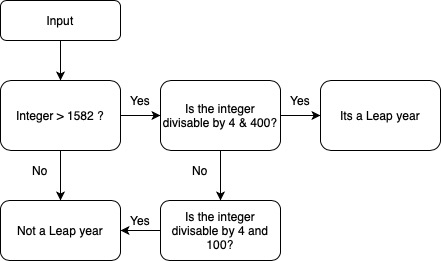
\includegraphics[scale=1]{FlowcharLeapYear.jpg}

The user inputs a value. If the value is less than 1582, the program will fail as a leap year and terminate the program. If it is higher, the it will pass. If the integer is divisible by 4 & 400, it will pass as a leap year, if not i will go through a last check. If the integer is divisible by 4 and 100, it was fail as a leap year. Else it is.


\end{document}

